% Usage: knitr slide


\def\apacue{1}
\chapter{Analysis of Covariance in Randomized Studies}\label{chap:ancova}

{\smaller[-1] \textbf{Hierarchy of Causal Inference for Treatment Efficacy}}

\bigskip

Let $P_{i}$ denote patient $i$ and the treatments be denoted by $A$
and $B$.  Thus $P_{2}^{B}$ represents patient 2 on treatment $B$.
$\overline{P}_{1}$ represents the average outcome over a sample of
patients from which patient 1 was selected.

\medskip

\begin{tabular}{ll}
\textbf{Design} & \textbf{Patients Compared} \\ \hline
6-period crossover & $P_{1}^{A}$ vs $P_{1}^{B}$ (directly measure HTE)\\
2-period crossover & $P_{1}^{A}$ vs $P_{1}^{B}$ \\
RCT in idential twins & $P_{1}^{A}$ vs $P_{1}^{B}$ \\
$\parallel$ group RCT & $\overline{P}_{1}^{A}$ vs $\overline{P}_{2}^{B}$, 
$P_{1}=P_{2}$ on avg \\
Observational, good artificial control & $\overline{P}_{1}^{A}$ vs 
$\overline{P}_{2}^{B}$, $P_{1}=P_{2}$ hopefully on avg\\
Observational, poor artificial control & $\overline{P}_{1}^{A}$ vs 
$\overline{P}_{2}^{B}$, $P_{1}\neq P_{2}$ on avg\\
Real-world physician practice & $P_{1}^{A}$ vs $P_{2}^{B}$ \\
 \hline
\end{tabular}


\section{Covariable Adjustment in Linear
  Models}\sound{anc-1}\disc{ancova-linear} 
\bi
\item   Model: $E(Y | X) = X \beta + \epsilon$
\item   Continuous response variable $Y$, normal residuals
\item   Statistical testing for baseline differences is scientifically
        incorrect (Altman \& Dor\'{e} 1990, Begg 1990, Senn 1994,
        Austin~\etal\ 2010); as Bland and Altman
        stated~\cite{bla11com}, statistical tests draw inferences
        about \emph{populations}, and the population model here would
        involve a repeat of the randomization to the whole population
        hence balance would be perfect.  Therefore the null hypothesis of no
        difference in baseline distributions between treatment groups
        is automatically true.
\item   If we are worried about baseline imbalance we need to search
        patient records for counter-- balancing factors
\item   \ra imbalance is not the reason to adjust for covariables
\item   Adjust to gain efficiency by subtracting explained variation
\item   Relative efficiency of unadjusted treatment comparison is $1-\rho^2$
\item   Unadjusted analyses yields unbiased treatment effect estimate
\ei

\section{Covariable Adjustment in Nonlinear Models}\sound{anc-2}\disc{ancova-nonlin}
\subsection{Hidden Assumptions in $2 \times 2$ Tables}
\bi
\item   Traditional presentation of 2--treatment clinical trial with a
        binary response: $2 \times 2$ table
\item   Parameters: $P_{1}, P_{2}$ for treatments 1, 2
\item   Test of goodness of fit: $H_0$: all patients in one treatment
        group have same probability of positive response ($P_j$ constant)
\item   \ra $H_0$: no risk factors exist
\item   Need to account for patient heterogeneity
\item   \cite{mat15inc} has a method for estimating the bias in
  unadjusted the log odds ratio and also has excellent background information
\ei

\subsection{Models for Binary Response}
\bi
\item   Model for probability of event must be nonlinear in predictors
        unless risk range is tiny
\item   Useful summary of relative treatment effect is the odds ratio (OR)
\item   Use of binary logistic model for covariable adjustment will
        result in an {\bf increase} in the S.E. of the treatment
        effect (log odds ratio) (Robinson \& Jewell, \cite{rob91som})
\item   But even with perfect balance, adjusted OR $\neq$ unadjusted
        OR
\item   Adjusted OR will be greater than unadjusted OR
\ei

\subsubsection{Example from GUSTO--I}\label{sec:ancova-gusto}\sound{anc-3}
\bi
\item   Steyerberg, Bossuyt, Lee \cite{ste00cli}
\item   Endpoint: 30--day mortality (0.07 overall)
\item   10,348 patients given accelerated $t$--PA
\item   20,162 patients given streptokinase (SK)
\item   Means and Percentages
\ei

{\smaller
\btable{lcc}{Characteristics of 30,000 GUSTO Patients} \hline\hline
Baseline Characteristic &   $t$--PA     &   SK  \\ \hline
Age             &   ~61.0   & ~60.9 \\
Female          &   ~25.3   & ~25.3 \\
Weight          &   ~79.6   & ~79.4 \\
Height          &   171.1   & 171.0 \\
Hypertension    &   ~38.2   & ~38.1 \\
Diabetes        &   ~14.5   & ~15.1 \\
Never smoked    &   ~29.8   & ~29.6 \\
High cholesterol&   ~34.6   & ~34.3 \\
Previous MI     &   ~16.9   & ~16.5 \\
Hypotension     &   ~~8.0   & ~~8.3 \\
Tachycardia     &   ~32.5   & ~32.7 \\
Anterior MI     &   ~38.9   & ~38.9 \\
Killip class I  &   ~85.0   & ~85.4 \\
ST elevation    &   ~37.3   & ~37.8 \\ \hline
\etable}

\subsubsection{Unadjusted / Adj.\ Logistic Estimates}
\bi
\item   With and without adjusting for 17 baseline characteristics
\btable{lccc}{Unadjusted and Adjusted GUSTO Analyses} \hline\hline
Type of Analysis    &   Log OR          &   S.E.    & $\chi^2$ \\ \hline
Unadjusted          &   -0.159          &   0.049   & 10.8 \\
Adjusted            &   -0.198          &   0.053   & 14.0 \\ \hline
\etable
\item   Percent reduction in odds of death: 15\% vs.\ 18\%
\item   -0.159 (15\%) is a biased estimate
\item   Increase in S.E.\ more than offset by increase in treatment effect
\item   Adjusted comparison based on 19\% fewer patients would have
        given same power as unadjusted test
\begin{Schunk}
\begin{Sinput}
load('gustomin.rda')
with(gustomin,
     plot(density(p.sk), xlim=c(0, .4), xlab='Baseline Expected Risk',
          ylab='Probability Density', main='') )    # Fig. (*\ref{fig:ancova-gustohistrisk}*)
\end{Sinput}
\begin{figure}[htbp]

\centerline{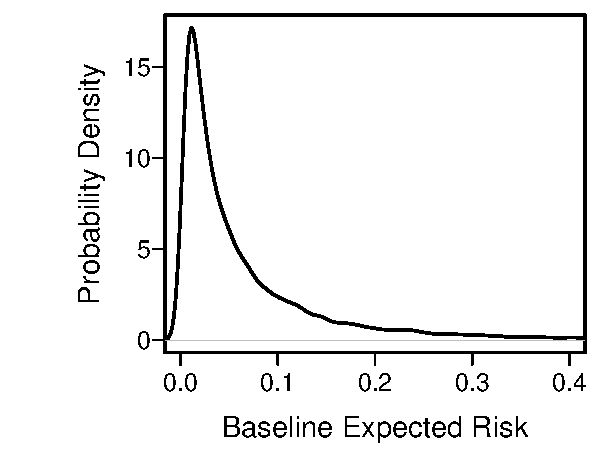
\includegraphics{ancova-gustohistrisk-1} }

\caption[Distribution of baseline risk in GUSTO-I]{Distribution of baseline risk in GUSTO-I.  Kernel density estimate of risk distribution for SK treatment.  Average risk is 0.07.  See also \cite{ioa97imp}.}\label{fig:ancova-gustohistrisk}
\end{figure}
\end{Schunk}
\item   Robinson \& Jewell: ``It is always more efficient to adjust \ipacue
        for predictive covariates when logistic models are used, and thus in
        this regard the behavior of logistic regression is the same as that of
        classic linear regression.''
\ei

\subsubsection{Simple Logistic Example -- Gail 1986}
\newcommand{\subtab}[6]{\begin{center}\begin{tabular}{l|c|c|}
    \multicolumn{3}{c}{#1} \\
    & Treatment A   & Treatment B \\ \hline
    $Y=1$ & #2 & #3 \\ \hline
    $Y=0$ & #4 & #5 \\ \hline
          & 1000 & 1000 \\
    \end{tabular}
    \\ Odds Ratio: #6
    \end{center}}
\subtab{Male}{500}{100}{500}{900}{9}
\subtab{Female}{900}{500}{100}{500}{9}
\subtab{Pooled}{1400}{600}{600}{1400}{5.44}

From seeing this example one can argue that odds ratios, like hazard
ratios, were never really designed to be computed on a set of subjects
having heterogeneity in their expected outcomes.

\subsection{Nonlinear Models, General}\sound{anc-4}
\bi
\item   Gail, Wieand, Piantadosi~\cite{gai84bia} showed that for unadjusted
        treatment estimates to be unbiased, regression must be linear
        or exponential
\item   Gail~\cite{gai86adj} showed that for logistic, Cox, and paired survival
        models unadjusted treatment effects are asymptotically biased
        low in absolute value
\item   Gail also studied normal, exponential, additive risk, Poisson
\ei
\quoteit{Part of the problem with
Poisson, proportional hazard and logistic regression approaches is
that they use a single parameter, the linear predictor, with no
equivalent of the variance parameter in the Normal case.  This means
that lack of fit impacts on the estimate of the
predictor.}{\citet{sen04con}, p. 3747}


\section{Cox / Log--Rank Test for Time to
  Event}\disc{ancova-efficiency} 
\bi
\item   Lagakos \& Schoenfeld 1984 showed that type I error is
        preserved if don't adjust
\item   If hazards are proportional conditional on covariables, they
        are not proportional if omit covariables
\item   Morgan 1986 derived asymptotic relative efficiencies (ARE) of
        unadjusted log--rank test if a binary covariable is omitted
\item   If prevalence of covariable $X$ is 0.5:
\ei
\btable{cc}{Efficiency of Unadjusted Log--Rank Test} \hline\hline
$X=1 : X=0$ Hazard Ratio    & ARE \\ \hline
1.0 &   1.00    \\
1.5 &   0.95    \\
2.0 &   0.88    \\
3.0 &   0.72    \\ \hline
\etable
\bi
\item   Ford, Norrie, Ahmadi~\cite{for95mod}: Treatment effect does not have the
        same interpretation under unadjusted and adjusted models
\item   No reason for the two hazard ratios to have the same value
\item   Akazawa, Nakamura, Palesch~\cite{aka97pow}: Power of unadjusted and
        stratified log--rank test
\ei
\btable{cccc}{Power With and Without Adjustment} \hline\hline
Number      &   Range of    &   \multicolumn{2}{c}{Power} \\
of Strata   &   Log Hazards &   Unadj.      &   Adjusted \\ \hline
1           &   0           &   .78         &   --  \\ \hline
2           &   0--0.5      &   .77         &   .78 \\
            &   0--1        &   .67         &   .78 \\
            &   0--2        &   .36         &   .77 \\ \hline
4           &   0--3        &   .35         &   .77 \\ \hline
8           &   0--3.5      &   .33         &   .77 \\ \hline
\etable

\subsection{Sample Size Calculation Issues}
\bi
\item   Schoenfeld~\cite{sch83sam} implies that covariable adjustment can only
        $\uparrow$ sample size in randomized trials
\item   Need to recognize ill--definition of unadjusted hazard ratios
\ei

\section{Why are Adjusted Estimates
  Right?}\sound{anc-5}\disc{ancova-meaning} 
\bi
\item   Hauck, Anderson, Marcus~\cite{hau98sho}, who have an excellent
        review of covariable adjustment in nonlinear models, state:
\begin{quote}\smaller
``For use in a clinician--patient
context, there is only a single person, that
patient, of interest.  The subject-specific measure
then best reflects the risks or benefits for that
patient.  Gail has noted this previously [ENAR
Presidential Invited Address, April 1990], arguing
that one goal of a clinical trial ought to be to
predict the direction and size of a treatment
benefit for a patient with specific covariate
values.  In contrast, population--averaged estimates
of treatment effect compare outcomes in groups of
patients.  The groups being compared are determined
by whatever covariates are included in the model.
The treatment effect is then a comparison of average
outcomes, where the averaging is over all omitted
covariates.''
\end{quote}
\ei

\section{How Many Covariables to Use?}\disc{ancova-plan}
\bi
\item   Try to adjust for the bulk of the variation in
        outcome \cite{hau98sho,tuk93tig}
\item   Neuhaus \cite{neu98est}: ``to improve the efficiency of
                  estimated covariate effects of interest, analysts of
                  randomized clinical trial data should adjust for
                  covariates that are strongly associated with the
                  outcome''
\item Raab~\etal~\cite{raa00how} have more guidance for choosing covariables and provide a formula for linear model that shows how the value of adding a covariable depends on the sample size
\ei

\section{Differential and Absolute Treatment Effects}\sound{anc-6}
\subsection{Modeling Differential Treatment Effect}\blog{2017/01/randomized-clinical-trials-do-not-mimic.html}\disc{ancova-hte}
Differential treatment effect is often called \emph{heterogeneity of
  treatment effect} or HTE.  As opposed to the natural expansion of
absolute treatment effect with underlying subject risk, differential
treatment effect is usually based on analyses of relative effects, especially
when the outcome is binary.

The most common approach to analyzing differential treatment effect
involves searching for such effects rather than estimating the
differential effect.  This is, tragically, most often done through
subgroup analysis.

\subsubsection{Problems With Subgroup Analysis}
\bi
\item   Subgroup analysis is widely practiced and widely derided in
  RCTs (as well as in observational studies)
\item Construction of a subgroup from underlying factors that are
  continuous in nature (e.g., ``older'' = age $\geq 65$) assumes that
  the treatment effect is like falling off a cliff, i.e.,
  all-or-nothing.  Discontinuous treatment effects, like discontinuous
  main effects, have not been found and validated but have always been
  shown to have been an artificial construct driven by opinion and not data.
\item Given a subgroup a simple label such as ``class IV heart
  failure'' may seem to be meaningful but subgrouping carries along other
  subject characteristics that are correlated with the subgrouping
  variable.  So the subgroup's treatment effect estimate has a more
  complex interpretation than what is thought.
\item Researchers who don't understand that ``absence of evidence is
  not evidence for absence'' interpret a significant effect in one
  subgroup but not in another as the treatment being effective in the
  first but ineffective in the second.  The second $P$-value may be
  large because of increased variability in the second subgroup or
  because of a smaller effective sample size in that group.
\item Testing the treatment effect in a subgroup does not carry along
  with it the covariate adjustment needed and assumes there is no
  residual HTE \emph{within} the subgroup.
\item When treatment interacts with factors not used in forming the
  subgroup, or when the subgrouping variable interacts with an
  ignored patient characteristic, the subgroup
  treatment effect may be grossly misleading.  As an example, in
  GUSTO-I there was a strong interaction between Killip class and
  age.  Unadjusted analysis of treatment effect within older subjects was
  partially an analysis of Killip class.  And the treatment effect was
  not ``significant'' in older patients, leading many readers to
  conclude $t$--PA should not be given to them.  In fact
  there was no evidence that age interacted with treatment, and the
  absolute risk reduction due to $t$--PA \emph{increased} with age.
\ei

\subsubsection{Specifying Interactions}\sound{anc-7}
\bi
\item   Assessing differential treatment effect best done with formal
        interaction tests rather than subgroup analysis
\item   Pre--specify sensible effect modifiers
    \bi
    \item   interactions between treatment and extent of disease
    \item   ``learned'' interventions: interaction between treatment
            and duration of use by physician
    \ei
\item   Interactions with center are not necessarily sensible
\item   Need to use penalized estimation (e.g., interaction effects as
        random effects) to get sufficient precision of differential
        treatment effects, if \# interaction d.f. $> 4$ for example
        \cite{sar96hie,yam99inv} \ipacue
\ei
\figs{cox-cabg-hazard-ratio}{A display of an interaction between treatment, extent of disease, and calendar year of start of treatment \cite{cal89}}{1}

\subsubsection{Strategy for Analyzing Differential Treatment Effect}\sound{anc-8}
The broad strategy that is recommended is based on the following:
\bi
\item Anything resembling subgroup analysis should be avoided
\item Anything that assumes that the treatment effect has a
  discontinuity in a continuous variable should be avoided.
  Differential effects should be smooth dose-response effects.
\item Anything that results in a finding that has a simpler alternate
  explanation should be avoided
  \bi
  \item Specify models so that an apparent interaction is not just a
    stand-in for an omitted main effect
  \ei
\ei
Particulars of the strategy are:
\bi
\item Formulate a subject-matter driven covariate model, including all
  covariates understood to have strong effects on the outcome.  Ensure
  that these covariates are adjusted for in every HTE analysis context.
\item Main effects need to be flexibly modeled (e.g., using regression
  splines) so as to not assume linearity.  False linearity assumptions
  can inflate apparent interaction effects because the interaction may
  be co-linear with omitted nonlinear main effects.
\item If the sample size allows, also model interaction effects as
  smooth nonlinear functions.  As with main effects, it is not
  uncommon for interaction effects to be nonlinear, e.g., the effect
  of treatment is small for age $<70$ then starts to expand rapidly
  after age 70\footnote{This does not imply that age should be modeled
    as a categorical variable to estimate the interaction; that would
    result in unexplained HTE in the age $\geq 70$ interval.}.  As a
  compromise, force interactions to be linear even if main effects are
  not, if the effective sample size does not permit estimating
  parameters for nonlinear differential effects.
\item Consider effect modifiers that are somewhat uncorrelated with
  each other.  Add the main effects corresponding to each potential
  effect modifier into the model described in the previous point.  For
  example if the primary analysis uses a model containing age, sex,
  and severity of disease and one is interested in assessing HTE by
  race and by geographical region, add \emph{both} race and region to the
  main effects that are adjusted for in \emph{all} later models.  This
  will result in proper covariate adjustment and will handle the case
  where an apparent interaction is partially explained by an omitted
  main effect that is co-linear with one of the interacting factors.
\item Carry out a joint (chunk) likelihood ratio or $F$-test for all \ipacue
  potential interaction effects combined.  This test has a perfect
  multiplicity adjustment and will not be ``brought down'' by the
  potential interactions being co-linear with each other.  The
  $P$-value from this joint test with multiple degrees of freedom will
  place the tests described in the next step in context.  But note
  that with many d.f.\ the test may lack power.
\item Consider each potential interaction one-at-a-time by adding that
  interaction term to the \emph{comprehensive} main effects model.  In
  the example given above, main effects simultaneously adjusted for
  would include treatment, age, sex, severity of disease, race, and
  region.  Then treatment $\times$ race is added to the model and
  tested.  Then the race interaction term (but not its main effect) is
  removed from the model and is replaced by region interactions.
\ei
Concerning the last step, we must really recognize that there are two
purposes for the analysis of differential treatment effect:
\be
\item Understanding which subject characteristics are associated with
  alterations in efficacy
\item Predicting the efficacy for an individual subject
\ee
For the latter purpose, one might include all potential treatment
interactions in the statistical model, whether interactions for
multiple baseline variables are co-linear or not.  Such co-linearities
do not hurt predictions or confidence intervals for predictions.  For
the former purpose, interactions can make one effect modifier compete
with another, and neither modifier will be significant when adjusted
for the other.  As an example, suppose that the model had main effects
for treatment, age, sex, and systolic and diastolic blood pressure
(SBP, DBP) and we entertained effect modification due to one or both
of SBP, DBP.  Because of the correlation between SBP and DBP, the main
effects for these variables are co-linear and their statistical
significance is weakened because they estimate, for example, the
effect of increasing SBP holding DBP constant (which is difficult to
do).  Likewise, treatment $\times$ SBP and treatment $\times$ DBP
interactions are co-linear with each other, making statistical tests
for interaction have low power.  We may find that neither SBP nor DBP
interaction is ``significant'' after adjusting for the other, but that
the combined chunk test for SBP or DBP interaction is highly
significant.  Someone who does not perform the chunk test may falsely
conclude that SBP does not modify the treatment effect.
This problem is more acute when more than two factors are allowed to
interact with treatment.

Note that including interaction terms in the model makes all treatment
effect estimates conditional on specific covariate values, effectively
lowering the sample size for each treatment effect estimate.  When
there is no HTE, the overall treatment main effect without having interaction
terms in the model is by far the highest precision estimate.  There is
a bias-variance tradeoff when considering HTE.  Adding interaction
terms lowers bias but greatly increases variance.

Another way to state the HTE estimation strategy is as follows.
\be
\item Pick a model for which it is mathematically possible that there
  be no interactions (no restrictions on model parameters)
\item Develop a model with ample flexibly-modeled main effects and
  clinically pre-specified interactions.  Use a Bayesian skeptical
  prior or penalized maximum likelihood estimate to shrink the
  interaction terms if the effective sample size does not support the
  pre-specified number of interaction parameters.  Be sure to model
  interaction effects as continuous if they come from variables of an
  underlying continuous nature.
\item Display and explain relative effects (e.g., odds ratios) as a
  function of interacting factors and link that to what is known about
  the mechanism of treatment effect.
\item Put all this in a context (like Figure~\ref{fig:ancova-ordiff})
  that shows absolute treatment benefit (e.g., risk scale) as a
  function of background risk and of interacting factors.
\item State clearly that background risk comes from all non-treatment
  factors and is a risk-difference accelerator that would increase
  risk differences for any risk factor, not just treatment.  Possibly
  provide a risk calculator to estimate background risk to plug into
  the $x$-axis.
\ee

Consider simulated two-treatment clinical trial data to illustrate the ``always adjust for all main effects but consider interactions one at a time'' approach to analyzing and displaying evidence for differential treatment effec.  After that we will illustrate a simultaneous interaction analysis.  Simulate time-to-event data from an exponential distribution, and fit Cox proportional hazards models to estimate the interaction between age and treatment and between sex and treatment.  The true age effect is simulated as linear in the log hazard and the treatment effect on the log relative hazard scale is proportional to how far above 60 years is a patient's age, with no treatment benefit before age 60.  This is a non-simple interaction that could be exactly modeled with a linear spline function, but assume that the analyst does not know the true form of the interaction so she allows for a more general smooth form using a restricted cubic spline function.  The data are simulated so that there is no sex interaction.

\begin{Sinput}
require(rms)
\end{Sinput}
\begin{Sinput}
options(prType='latex')   # for cph print, anova
set.seed(1)
n <- 3000    # total of 3000 subjects
age <- rnorm(n, 60, 12)
label(age) <- 'Age'
sex   <- factor(sample(c('Male', 'Female'), n, rep=TRUE))
treat <- factor(sample(c('A', 'B'), n, rep=TRUE))
cens  <- 15 * runif(n)     # censoring time
h <- 0.02 * exp(0.04 * (age - 60) + 0.4 * (sex == 'Female') -  
                0.04 * (treat == 'B') * pmax(age - 60, 0))
dt <- -log(runif(n)) / h
label(dt) <- 'Time Until Death or Censoring'
e <- ifelse(dt <= cens, 1, 0)
dt <- pmin(dt, cens)
units(dt) <- 'Year'
dd <- datadist(age, sex, treat); options(datadist='dd')
S <- Surv(dt, e)
f <- cph(S ~ sex + rcs(age, 4) * treat)
f
\end{Sinput}

 \centerline{\textbf{Cox Proportional Hazards Model}}
 
 \begin{verbatim}
 cph(formula = S ~ sex + rcs(age, 4) * treat)
 \end{verbatim}
 
 {\fontfamily{phv}\selectfont \begin{center}\begin{tabular}{|c|c|c|}\hline
&Model Tests&Discrimination\\
&&Indexes\\\hline
Obs~\hfill 3000&LR $\chi^{2}$~\hfill 126.48&$R^{2}$~\hfill 0.046\\
Events~\hfill 456&d.f.~\hfill 8&$D_{xy}$~\hfill 0.292\\
Center~\hfill 1.5014&Pr$(>\chi^{2})$~\hfill 0.0000&$g$~\hfill 0.556\\
&Score $\chi^{2}$~\hfill 148.58&$g_{r}$~\hfill 1.743\\
&Pr$(>\chi^{2})$~\hfill 0.0000&\\
\hline
\end{tabular}
\end{center}}
 
 %latex.default(U, file = "", first.hline.double = FALSE, table = FALSE,     longtable = TRUE, lines.page = lines.page, col.just = rep("r",         ncol(U)), rowlabel = "", already.math.col.names = TRUE,     append = TRUE)%
 \setlongtables\begin{longtable}{lrrrr}\hline
 \multicolumn{1}{l}{}&\multicolumn{1}{c}{$\hat{\beta}$}&\multicolumn{1}{c}{S.E.}&\multicolumn{1}{c}{Wald $Z$}&\multicolumn{1}{c}{Pr$(>|Z|)$}\tabularnewline
 \hline
 \endhead
 \hline
 \endfoot
 sex=Male&~-0.3794~&~0.0958~&-3.96&\textless 0.0001\tabularnewline
 age&~ 0.0269~&~0.0239~& 1.13&0.2605\tabularnewline
 age'&~ 0.0542~&~0.0587~& 0.92&0.3556\tabularnewline
 age''&~-0.2361~&~0.2315~&-1.02&0.3077\tabularnewline
 treat=B&~ 0.0218~&~1.6648~& 0.01&0.9895\tabularnewline
 age $\times$ treat=B&~-0.0008~&~0.0353~&-0.02&0.9815\tabularnewline
 age' $\times$ treat=B&~-0.0650~&~0.0890~&-0.73&0.4650\tabularnewline
 age'' $\times$ treat=B&~ 0.2525~&~0.3579~& 0.71&0.4805\tabularnewline
 \hline
 \end{longtable}
 \addtocounter{table}{-1}
\begin{Sinput}
anova(f)
\end{Sinput}
%latex.default(dstats, title = title, caption = if (table.env) caption else NULL,     insert.top = if (length(caption) && !table.env) paste0("\\Needspace{2in}\n",         caption), rowlabel = "", col.just = rep("r", length(sn)),     table.env = table.env, ...)%
\textbf{\Needspace{2in}
Wald Statistics for \texttt{\smaller S}}\begin{center}
\begin{tabular}{lrrr}
\hline\hline
\multicolumn{1}{l}{}&\multicolumn{1}{c}{$\chi^{2}$}&\multicolumn{1}{c}{d.f.}&\multicolumn{1}{c}{$P$}\tabularnewline
\hline
sex& 15.70&1&\textless 0.0001\tabularnewline
age  (Factor+Higher Order Factors)& 81.64&6&\textless 0.0001\tabularnewline
~~\emph{All Interactions}&  9.97&3&0.0188\tabularnewline
~~\emph{Nonlinear (Factor+Higher Order Factors)}&  1.41&4&0.8430\tabularnewline
treat  (Factor+Higher Order Factors)& 33.82&4&\textless 0.0001\tabularnewline
~~\emph{All Interactions}&  9.97&3&0.0188\tabularnewline
age $\times$ treat  (Factor+Higher Order Factors)&  9.97&3&0.0188\tabularnewline
~~\emph{Nonlinear}&  0.54&2&0.7651\tabularnewline
~~\emph{Nonlinear Interaction : f(A,B) vs. AB}&  0.54&2&0.7651\tabularnewline
TOTAL NONLINEAR&  1.41&4&0.8430\tabularnewline
TOTAL NONLINEAR + INTERACTION& 10.59&5&0.0600\tabularnewline
TOTAL&134.12&8&\textless 0.0001\tabularnewline
\hline
\end{tabular}\end{center}

The model fitted above allows for a general age $\times$ treatment interaction.  Let's explore this interaction by plotting the age effect separately by treatment group, then plotting the treatment B:A hazard ratio as a function of age.
\begin{Schunk}
\begin{Sinput}
ggplot(Predict(f, age, treat), rdata=data.frame(age, treat))
ages <- seq(30, 87, length=200)
k <- contrast(f, list(treat='B', age=ages), list(treat='A', age=ages))
class(k) <- 'data.frame'
ggplot(k, aes(x=age, y=exp(Contrast))) + scale_y_log10(minor_breaks=seq(.2, .9, by=.1)) + 
  geom_ribbon(aes(ymin=exp(Lower), ymax=exp(Upper)), fill='gray80') +
  geom_line() +
  ylab('B:A Hazard Ratio') + xlab('Age')
\end{Sinput}


\centerline{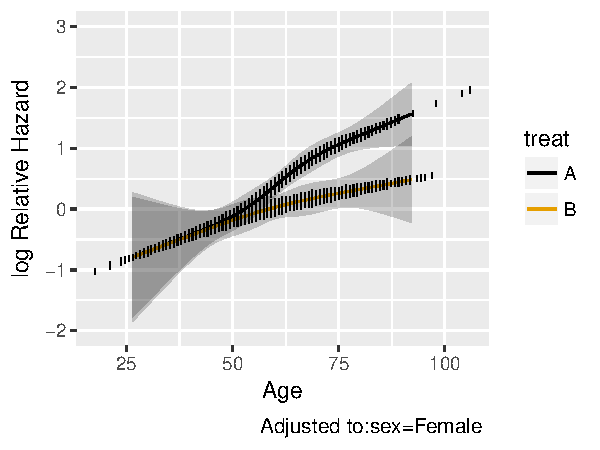
\includegraphics{ancova-hteplot-1} 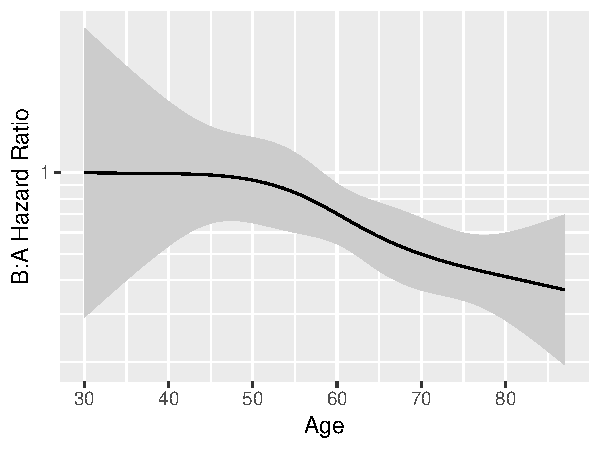
\includegraphics{ancova-hteplot-2} }

\end{Schunk}

Re-fit the model allowing for a sex interaction (but not an age interaction) and display the results.
\begin{Sinput}
g <- cph(S ~ sex * treat + rcs(age, 4))
g
\end{Sinput}

 \centerline{\textbf{Cox Proportional Hazards Model}}
 
 \begin{verbatim}
 cph(formula = S ~ sex * treat + rcs(age, 4))
 \end{verbatim}
 
 {\fontfamily{phv}\selectfont \begin{center}\begin{tabular}{|c|c|c|}\hline
&Model Tests&Discrimination\\
&&Indexes\\\hline
Obs~\hfill 3000&LR $\chi^{2}$~\hfill 116.79&$R^{2}$~\hfill 0.043\\
Events~\hfill 456&d.f.~\hfill 6&$D_{xy}$~\hfill 0.285\\
Center~\hfill 1.3019&Pr$(>\chi^{2})$~\hfill 0.0000&$g$~\hfill 0.603\\
&Score $\chi^{2}$~\hfill 118.46&$g_{r}$~\hfill 1.828\\
&Pr$(>\chi^{2})$~\hfill 0.0000&\\
\hline
\end{tabular}
\end{center}}
 
 %latex.default(U, file = "", first.hline.double = FALSE, table = FALSE,     longtable = TRUE, lines.page = lines.page, col.just = rep("r",         ncol(U)), rowlabel = "", already.math.col.names = TRUE,     append = TRUE)%
 \setlongtables\begin{longtable}{lrrrr}\hline
 \multicolumn{1}{l}{}&\multicolumn{1}{c}{$\hat{\beta}$}&\multicolumn{1}{c}{S.E.}&\multicolumn{1}{c}{Wald $Z$}&\multicolumn{1}{c}{Pr$(>|Z|)$}\tabularnewline
 \hline
 \endhead
 \hline
 \endfoot
 sex=Male&~-0.3333~&~0.1222~&-2.73&0.0064\tabularnewline
 treat=B&~-0.4351~&~0.1249~&-3.48&0.0005\tabularnewline
 age&~ 0.0264~&~0.0176~& 1.50&0.1337\tabularnewline
 age'&~ 0.0293~&~0.0441~& 0.67&0.5060\tabularnewline
 age''&~-0.1387~&~0.1759~&-0.79&0.4304\tabularnewline
 sex=Male $\times$ treat=B&~-0.1217~&~0.1963~&-0.62&0.5354\tabularnewline
 \hline
 \end{longtable}
 \addtocounter{table}{-1}
\begin{Sinput}
anova(g)
\end{Sinput}
%latex.default(dstats, title = title, caption = if (table.env) caption else NULL,     insert.top = if (length(caption) && !table.env) paste0("\\Needspace{2in}\n",         caption), rowlabel = "", col.just = rep("r", length(sn)),     table.env = table.env, ...)%
\textbf{\Needspace{2in}
Wald Statistics for \texttt{\smaller S}}\begin{center}
\begin{tabular}{lrrr}
\hline\hline
\multicolumn{1}{l}{}&\multicolumn{1}{c}{$\chi^{2}$}&\multicolumn{1}{c}{d.f.}&\multicolumn{1}{c}{$P$}\tabularnewline
\hline
sex  (Factor+Higher Order Factors)& 16.19&2&0.0003\tabularnewline
~~\emph{All Interactions}&  0.38&1&0.5354\tabularnewline
treat  (Factor+Higher Order Factors)& 25.63&2&\textless 0.0001\tabularnewline
~~\emph{All Interactions}&  0.38&1&0.5354\tabularnewline
age& 72.80&3&\textless 0.0001\tabularnewline
~~\emph{Nonlinear}&  0.89&2&0.6420\tabularnewline
sex $\times$ treat  (Factor+Higher Order Factors)&  0.38&1&0.5354\tabularnewline
TOTAL NONLINEAR + INTERACTION&  1.27&3&0.7367\tabularnewline
TOTAL&111.89&6&\textless 0.0001\tabularnewline
\hline
\end{tabular}\end{center}
\begin{Sinput}
ggplot(Predict(g, sex, treat))
k <- contrast(g, list(treat='B', sex=levels(sex)), list(treat='A', sex=levels(sex)))
class(k) <- 'data.frame'
ggplot(k, aes(y=exp(Contrast), x=sex)) + geom_point() + scale_y_log10(breaks=c(.5, .6, .7, .8, .9, 1, 1.1)) +
  geom_linerange(aes(ymin=exp(Lower), ymax=exp(Upper))) + 
  xlab('Sex') + ylab('B:A Hazard Ratio') + coord_flip()
\end{Sinput}


\centerline{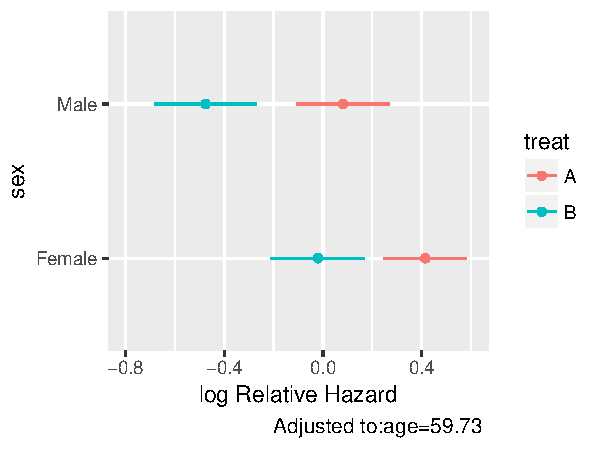
\includegraphics{ancova-hteplot2-1} 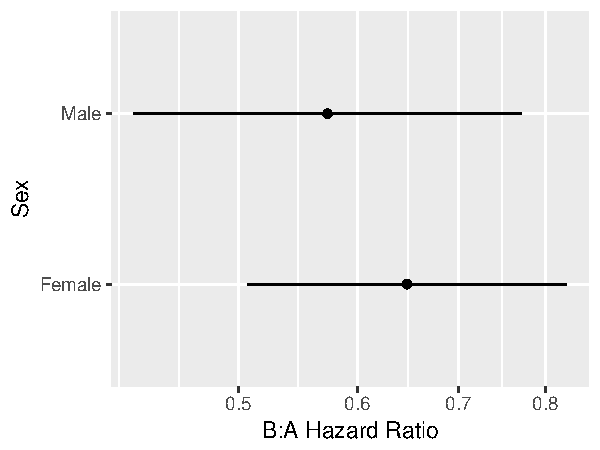
\includegraphics{ancova-hteplot2-2} }


The above analysis signified a treatment effect for both sex groups (both confidence limits exclude a hazard ratio of 1.0), whereas this should only be the case when age exceeds 60.  No sex $\times$ treatment interaction was indicated.
Re-do the previous analysis adjusting for an age $\times$ treatment interaction while estimating the sex $\times$ treatment interaction.  For this purpose we must specify an age value when estimating the treatment effects by sex.  Here we set age to 50 years.  Were age and sex correlated, the joint analysis would have been harder to interpret.
\begin{Sinput}
h <- cph(S ~ treat * (rcs(age, 4) + sex))
anova(h)
\end{Sinput}
%latex.default(dstats, title = title, caption = if (table.env) caption else NULL,     insert.top = if (length(caption) && !table.env) paste0("\\Needspace{2in}\n",         caption), rowlabel = "", col.just = rep("r", length(sn)),     table.env = table.env, ...)%
\textbf{\Needspace{2in}
Wald Statistics for \texttt{\smaller S}}\begin{center}
\begin{tabular}{lrrr}
\hline\hline
\multicolumn{1}{l}{}&\multicolumn{1}{c}{$\chi^{2}$}&\multicolumn{1}{c}{d.f.}&\multicolumn{1}{c}{$P$}\tabularnewline
\hline
treat  (Factor+Higher Order Factors)& 34.18&5&\textless 0.0001\tabularnewline
~~\emph{All Interactions}& 10.33&4&0.0353\tabularnewline
age  (Factor+Higher Order Factors)& 81.66&6&\textless 0.0001\tabularnewline
~~\emph{All Interactions}&  9.94&3&0.0191\tabularnewline
~~\emph{Nonlinear (Factor+Higher Order Factors)}&  1.36&4&0.8505\tabularnewline
sex  (Factor+Higher Order Factors)& 16.06&2&0.0003\tabularnewline
~~\emph{All Interactions}&  0.36&1&0.5502\tabularnewline
treat $\times$ age  (Factor+Higher Order Factors)&  9.94&3&0.0191\tabularnewline
~~\emph{Nonlinear}&  0.50&2&0.7788\tabularnewline
~~\emph{Nonlinear Interaction : f(A,B) vs. AB}&  0.50&2&0.7788\tabularnewline
treat $\times$ sex  (Factor+Higher Order Factors)&  0.36&1&0.5502\tabularnewline
TOTAL NONLINEAR&  1.36&4&0.8505\tabularnewline
TOTAL INTERACTION& 10.33&4&0.0353\tabularnewline
TOTAL NONLINEAR + INTERACTION& 10.95&6&0.0898\tabularnewline
TOTAL&133.11&9&\textless 0.0001\tabularnewline
\hline
\end{tabular}\end{center}
\begin{Sinput}
ggplot(Predict(h, sex, treat, age=50))
k <- contrast(h, list(treat='B', sex=levels(sex), age=50),
                 list(treat='A', sex=levels(sex), age=50))
class(k) <- 'data.frame'
ggplot(k, aes(y=exp(Contrast), x=sex)) + geom_point() + scale_y_log10(breaks=c(.5, .6, .7, .8, .9, 1, 1.1)) +
  geom_linerange(aes(ymin=exp(Lower), ymax=exp(Upper))) + 
  xlab('Sex') + ylab('B:A Hazard Ratio') + coord_flip()
\end{Sinput}


\centerline{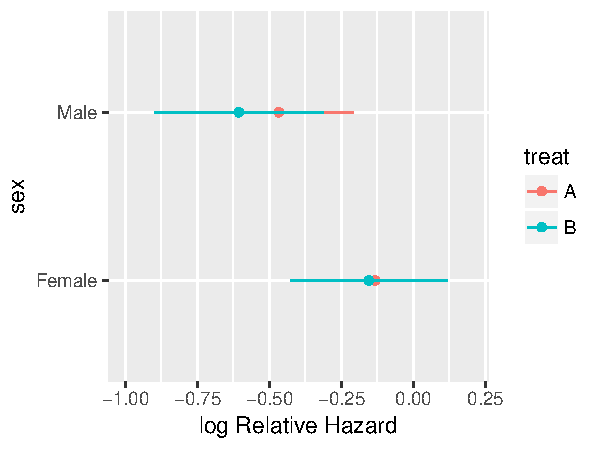
\includegraphics{ancova-htejoint-1} 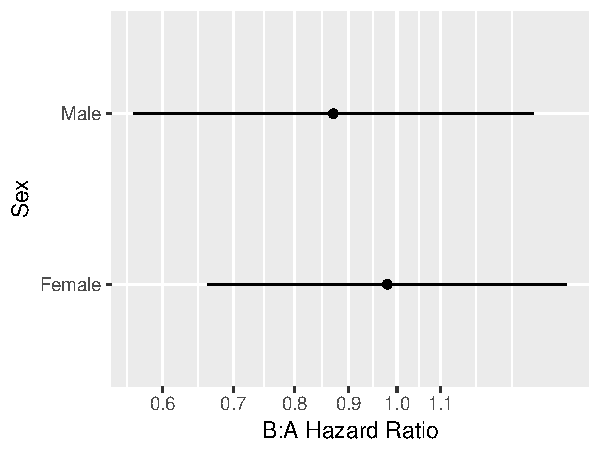
\includegraphics{ancova-htejoint-2} }


This is a more accurate representation of the true underlying model, and is easy to interpret because (1) age and sex are uncorrelated in the simulation model used, and (2) only two interactions were considered. 

\subsubsection{Absolute vs.\ Relative Treatment Effects Revisited}\sound{anc-9}\disc{ancova-absolute}
Statistical models are typically chosen so as to maximize the
likelihood of the model fitting the data and processes that generated
them.  Even though one may be interested in absolute effects, models
must usually be based on relative effects so that quantities such as
estimated risk are in the legal $[0,1]$ range.  It is not unreasonable
to think of a relative effects model such as the logistic model as
providing supporting evidence that an interacting effect \emph{causes}
a change in the treatment effect, whereas the necessary expansion of
treatment effect for higher risk subjects, as detailed in the next
section, is merely a mathematical necessity for how probabilities
work.  One could perhaps say that any factor that confers increased
risk for a subject (up to the point of diminishing returns; see below)
might \emph{cause} an increase in the treatment effect, but this is a
general phenomenon that is spread throughout all risk factors
independently of how they may directly affect the treatment effect.
Because of this, additive risk models are not recommended for modeling
outcomes or estimating differential treatment effects on an absolute
scale.  This logic leads to the following recommended strategy:
\be
\item Base all inference and predicted risk estimation on a model most
  likely to fit the data (e.g., logistic risk model; Cox model).
  Choose the model so that it is \emph{possible} that there may be no
  interactions, i.e., a model that does not place a restriction on
  regression coefficients.
\item Pre-specify sensible possible interactions as described earlier
\item Use estimates from this model to estimate relative differential
  treatment effects, which should be smooth functions of continuous
  baseline variables
\item Use the same model to estimate absolute risk differences (as in
  the next section) as a function both of interacting factors and of
  baseline variables in the model that do not interact with treatment
  (but will still expand the absolute treatment effect)
\item Even better: since expansion of risk differences is a general
  function of overall risk and not of individual risk factors only
  display effects of individual risk factors that interact with
  treatment (interacting on the scale that would have allowed them not
  to interact---the relative scale such as log odds) and show the
  general risk difference expansion as in Figures
  \ref{fig:ancova-or-diff} (think of the ``risk factor'' as treatment)
  and \ref{fig:ancova-gusto-nomogram}
\ee

\quoteit{To translate the results of clinical trials into practice may
  require a lot of work involving modelling and further background
  information.  `Additive at the point of analysis but relevant at the
  point of application' should be the motto.}{Stephen Senn in
\url{http://errorstatistics.com/2013/04/19/stephen-senn-when-relevance-is-irrelevant}}

\subsection{Estimating Absolute Treatment
  Effects}\sound{anc-10}\disc{ancova-absolute}
\bi
\item   Absolute efficacy measures:
    \bi
    \item   Risk difference ($\delta$)
    \item   number needed to treat (reciprocal of risk
        difference)
    \item   Years of life saved
    \item   Quality--adjusted life years saved
    \ei
\item   Binary response, no interactions with treatment, risk for
        control patient $P$: \\
        $\delta = P - \frac{P}{P + (1-P)/OR}$
\item   $\delta$ is dominated by $P$
\ei
\begin{Schunk}
\begin{Sinput}
plot(0, 0, type="n", xlab="Risk for Subject Without Risk Factor",
     ylab="Increase in Risk",
     xlim=c(0,1), ylim=c(0,.6))   # Figure (*\ref{fig:ancova-or-diff}\ipacue*)
i <- 0
or <- c(1.1,1.25,1.5,1.75,2,3,4,5,10)
for(h in or) {
  i <- i + 1
  p <- seq(.0001, .9999, length=200)
  logit <- log(p/(1 - p))  # same as qlogis(p)
  logit <- logit + log(h)  # modify by odds ratio
  p2 <- 1/(1 + exp(-logit))# same as plogis(logit)
  d <- p2 - p
  lines(p, d, lty=i)
  maxd <- max(d)
  smax <- p[d==maxd]
  text(smax, maxd + .02, format(h), cex=.6)
}
\end{Sinput}
\begin{figure}[htbp]

\centerline{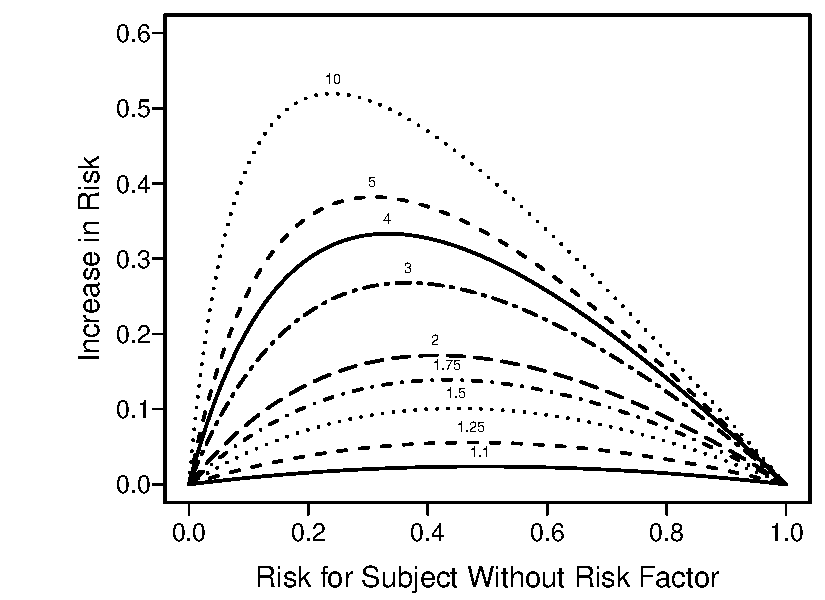
\includegraphics{ancova-or-diff-1} }

\caption[Absolute risk increase as a function of risk]{Absolute risk increase as a function of risk for control subject.  Numbers on curves are treatment:control odds ratios.}\label{fig:ancova-or-diff}
\end{figure}
\end{Schunk}
If the outcome is such that $Y=1$ implies a good outcome,
Figure~\ref{fig:ancova-or-diff} would be useful for estimating the
absolute risk increase for a ``good'' treatment by selecting the one
curve according to the odds ratio the treatment achieved in a
multivariable risk model.  This assumes that the treatment does not
interact with any patient characteristic(s).

van~Klaveren~et~al.~\cite{kla15est} described the importance of correctly modeling interactions when estimating absolute treatment benefit.

Now consider the case \sound{anc-11}
where $Y=1$ is a bad outcome and $Y=0$ is a good outcome, and there is
differential relative treatment effect according to a truly binary
patient characteristic $X=0,1$.  Suppose that treatment represents a
new agent and the control group is patients on standard therapy.
Suppose that the new treatment multiplies the odds of a bad outcome by
0.8 when $X=0$ and by 0.6 when $X=1$, and that the background risk
that $Y=1$ for patients on standard therapy ranges from 0.01 to 0.99.
The background risk could come from one or more continuous variables
or mixtures of continuous and categorical patient characteristics.
The ``main effect'' of $X$ must also be specified.  We assume that
$X=0$ goes into the background risk and $X=1$ increases the odds that
$Y=1$ by a factor of 1.4 for patients on standard therapy.
All of this specifies a full probability model that can be evaluated
to show the absolute risk reduction by the new treatment as a function
of background risk and $X$.

\begin{Schunk}
\begin{Sinput}
require(Hmisc)
d <- expand.grid(X=0:1, brisk=seq(0.01, 0.99, length=150))
d <- upData(d,
            risk.standard = plogis(qlogis(brisk) + log(1.4) * X),
            risk.new      = plogis(qlogis(brisk) + log(1.4) * X +
                                     log(0.8) * (X == 0) +
                                     log(0.6) * (X == 1)),
            risk.diff     = risk.standard - risk.new,
            X = factor(X) )
\end{Sinput}
\begin{Soutput}
Input object size:	 17640 bytes;	 2 variables	 300 observations
Added variable		risk.standard
Added variable		risk.new
Added variable		risk.diff
Modified variable	X
New object size:	25664 bytes;	5 variables	300 observations
\end{Soutput}
\begin{Sinput}
ggplot(d, aes(x=risk.standard, y=risk.diff, color=X)) +
  geom_line() +
  xlab('Risk Under Standard Treatment') +
  ylab('Absolute Risk Reduction With New Treatment')   # (*\ipacue*)
\end{Sinput}
\begin{figure}[htbp]

\centerline{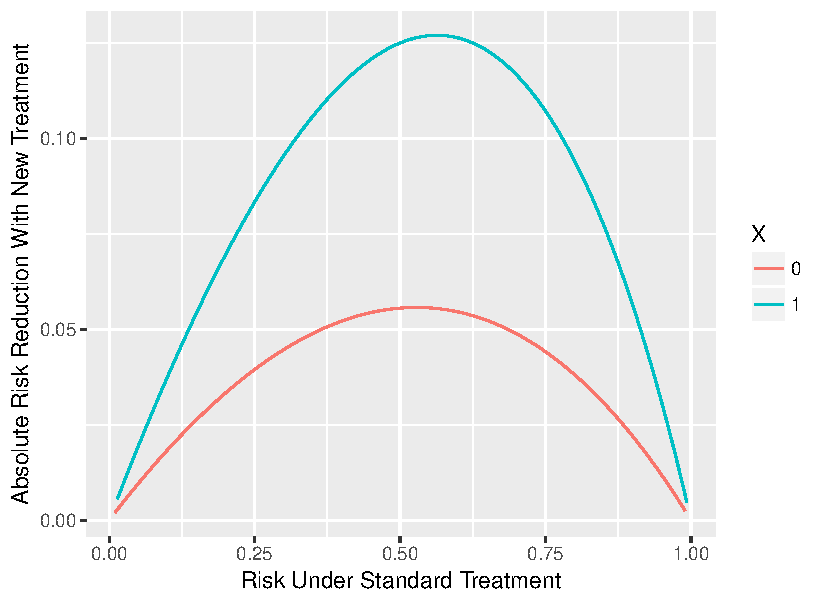
\includegraphics{ancova-ordiff-1} }

\caption[Absolute risk reduction by background risk and interacting factor]{Absolute risk reduction by a new treatment as a function of background risk and an interacting factor}\label{fig:ancova-ordiff}
\end{figure}
\end{Schunk}
It is important to note that the magnification of absolute risk
reduction by increasing background risk should not be labeled (or
analyzed) by any one contributing risk factor.  This is a generalized
effect that comes solely from the restriction of probabilities to the
$[0,1]$ range.


\subsubsection{Absolute Treatment Effects for GUSTO--I}\sound{anc-12}
\bi
\item   No evidence for interactions with treatment
\item   Misleading subgroup analysis showed that elderly patients not
        benefit from $t$--PA; result of strong age $\times$ Killip
        class interaction
\item   Wide variation in absolute benefit of $t$--PA \ipacue
\begin{Schunk}
\begin{Sinput}
delta <- with(gustomin, p.sk - p.tpa)
plot(density(delta), xlab='Mortality Difference',
     ylab='Probability Density', main='')    # Fig. (*\ref{fig:ancova-gusto-histdelt}*)
m <- mean(delta)
u <- par("usr")
arrows(m, u[3], m, 0, length=.1, lwd=2)
text(m, 2, 'Mean', srt=45, adj=0)
med <- median(delta)
arrows(med, u[3], med, 0, length=.1, lwd=2)
text(med, 2, 'Median', srt=45, adj=0)
\end{Sinput}
\begin{figure}[htbp]

\centerline{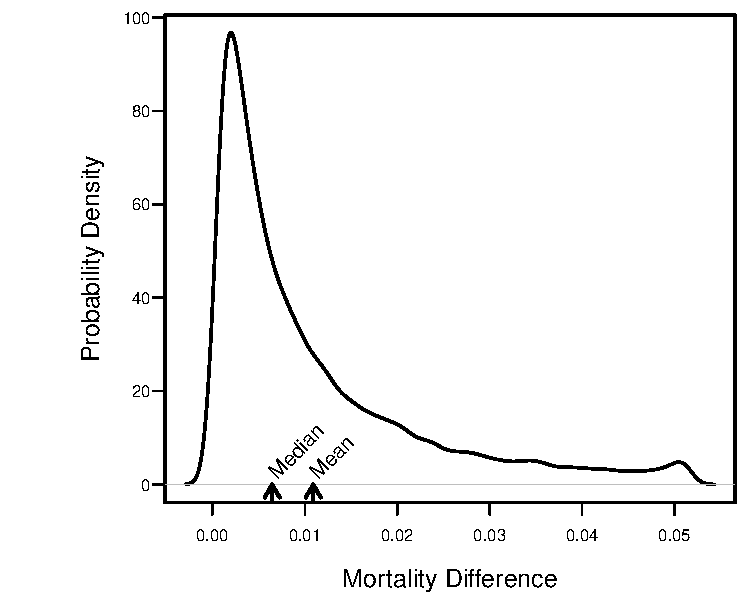
\includegraphics{ancova-gusto-histdelt-1} }

\caption[Absolute benefit vs.\ baseline risk]{Distribution of absolute risk reduction with $t$--PA vs.\ SK}\label{fig:ancova-gusto-histdelt}
\end{figure}
\end{Schunk}
\item   Overall mortality difference of 0.011 dominated by high--risk patients
\ei
\begin{Sinput}
load('gusto.rda')
require(rms)
dd <- datadist(gusto); options(datadist='dd')
f <- lrm(day30 ~ tx + age * Killip + pmin(sysbp, 120) +
           lsp(pulse, 50) + pmi + miloc, data=gusto)
cat('{\\smaller ')
\end{Sinput}
{\smaller \begin{Sinput}
f
\end{Sinput}

 \centerline{\textbf{Logistic Regression Model}}
 
 \begin{verbatim}
 lrm(formula = day30 ~ tx + age * Killip + pmin(sysbp, 120) + 
     lsp(pulse, 50) + pmi + miloc, data = gusto)
 \end{verbatim}
 
 {\fontfamily{phv}\selectfont \begin{center}\begin{tabular}{|c|c|c|c|}\hline
&Model Likelihood&Discrimination&Rank Discrim.\\
&Ratio Test&Indexes&Indexes\\\hline
Obs~\hfill 40830&LR $\chi^{2}$~\hfill 4173.41&$R^{2}$~\hfill 0.245&$C$~\hfill 0.821\\
~~0~\hfill 37979&d.f.~\hfill 15&$g$~\hfill 1.490&$D_{xy}$~\hfill 0.642\\
~~1~\hfill 2851&Pr$(>\chi^{2})$~\hfill \textless 0.0001&$g_{r}$~\hfill 4.437&$\gamma$~\hfill 0.642\\
$\max|\frac{\partial\log L}{\partial \beta}|$~\hfill $5\!\times\!10^{-6}$&&$g_{p}$~\hfill 0.083&$\tau_{a}$~\hfill 0.083\\
&&Brier~\hfill 0.055&\\
\hline
\end{tabular}
\end{center}}
 
 %latex.default(U, file = "", first.hline.double = FALSE, table = FALSE,     longtable = TRUE, lines.page = lines.page, col.just = rep("r",         ncol(U)), rowlabel = "", already.math.col.names = TRUE,     append = TRUE)%
 \setlongtables\begin{longtable}{lrrrr}\hline
 \multicolumn{1}{l}{}&\multicolumn{1}{c}{$\hat{\beta}$}&\multicolumn{1}{c}{S.E.}&\multicolumn{1}{c}{Wald $Z$}&\multicolumn{1}{c}{Pr$(>|Z|)$}\tabularnewline
 \hline
 \endhead
 \hline
 \endfoot
 Intercept&~-3.9541~&~0.7135~& -5.54&\textless 0.0001\tabularnewline
 tx=SK&~ 0.0738~&~0.0512~&  1.44&0.1499\tabularnewline
 tx=tPA&~-0.1338~&~0.0608~& -2.20&0.0276\tabularnewline
 age&~ 0.0867~&~0.0026~& 33.67&\textless 0.0001\tabularnewline
 Killip=II&~ 2.1146~&~0.3610~&  5.86&\textless 0.0001\tabularnewline
 Killip=III&~ 3.7596~&~0.7310~&  5.14&\textless 0.0001\tabularnewline
 Killip=IV&~ 4.0790~&~0.8259~&  4.94&\textless 0.0001\tabularnewline
 sysbp&~-0.0386~&~0.0017~&-23.10&\textless 0.0001\tabularnewline
 pulse&~-0.0221~&~0.0141~& -1.57&0.1168\tabularnewline
 pulse'&~ 0.0416~&~0.0143~&  2.90&0.0037\tabularnewline
 pmi=yes&~ 0.4664~&~0.0485~&  9.62&\textless 0.0001\tabularnewline
 miloc=Other&~ 0.3048~&~0.1163~&  2.62&0.0087\tabularnewline
 miloc=Anterior&~ 0.5370~&~0.0443~& 12.12&\textless 0.0001\tabularnewline
 age $\times$ Killip=II&~-0.0216~&~0.0051~& -4.22&\textless 0.0001\tabularnewline
 age $\times$ Killip=III&~-0.0363~&~0.0103~& -3.51&0.0004\tabularnewline
 age $\times$ Killip=IV&~-0.0323~&~0.0124~& -2.61&0.0090\tabularnewline
 \hline
 \end{longtable}
 \addtocounter{table}{-1}
\begin{Sinput}
anova(f)
\end{Sinput}
%latex.default(dstats, title = title, caption = if (table.env) caption else NULL,     insert.top = if (length(caption) && !table.env) paste0("\\Needspace{2in}\n",         caption), rowlabel = "", col.just = rep("r", length(sn)),     table.env = table.env, ...)%
\textbf{\Needspace{2in}
Wald Statistics for \texttt{\smaller day30}}\begin{center}
\begin{tabular}{lrrr}
\hline\hline
\multicolumn{1}{l}{}&\multicolumn{1}{c}{$\chi^{2}$}&\multicolumn{1}{c}{d.f.}&\multicolumn{1}{c}{$P$}\tabularnewline
\hline
tx&  15.46& 2&0.0004\tabularnewline
age  (Factor+Higher Order Factors)&1390.07& 4&\textless 0.0001\tabularnewline
~~\emph{All Interactions}&  31.13& 3&\textless 0.0001\tabularnewline
Killip  (Factor+Higher Order Factors)& 427.94& 6&\textless 0.0001\tabularnewline
~~\emph{All Interactions}&  31.13& 3&\textless 0.0001\tabularnewline
sysbp& 533.64& 1&\textless 0.0001\tabularnewline
pulse& 325.19& 2&\textless 0.0001\tabularnewline
~~\emph{Nonlinear}&   8.43& 1&0.0037\tabularnewline
pmi&  92.55& 1&\textless 0.0001\tabularnewline
miloc& 146.92& 2&\textless 0.0001\tabularnewline
age $\times$ Killip  (Factor+Higher Order Factors)&  31.13& 3&\textless 0.0001\tabularnewline
TOTAL NONLINEAR + INTERACTION&  39.17& 4&\textless 0.0001\tabularnewline
TOTAL&3167.41&15&\textless 0.0001\tabularnewline
\hline
\end{tabular}\end{center}
\begin{Sinput}
cat('}')   # (*\ipacue*)
\end{Sinput}
}\begin{Sinput}
cof <- coef(f)             # vector of regression coefficients
# For cof, X*beta without treatment coefficients estimates logit
# for SK+t-PA combination therapy (reference cell).  The coefficient for
# SK estimates the difference in logits from combo to SK.  The coefficient
# for tPA estimates the difference in tPA from combo.  The mortality
# difference of interest is mortality with SK minus mortality with tPA.
mort.sk   <- function(x) plogis(x + cof['tx=SK'])
mort.diff <- function(x)
  ifelse(x < 0, mort.sk(x) - plogis(x + cof['tx=tPA']), NA)
# only define when logit < 0 since U-shaped
n <- nomogram(f, fun=list(mort.sk, mort.diff),
              funlabel=c("30-Day Mortality\nFor SK Treatment",
                         "Mortality Reduction by t-PA"),
              fun.at=list(c(.001,.005,.01,.05,.1,.2,.5,.7,.9),
                c(.001,.005,.01,.02,.03,.04,.05)),
              pulse=seq(0,260,by=10), omit='tx', lp=FALSE)
plot(n, varname.label.sep=' ', xfrac=.27, lmgp=.2, cex.axis=.6)
\end{Sinput}
\begin{figure}[htbp]

\centerline{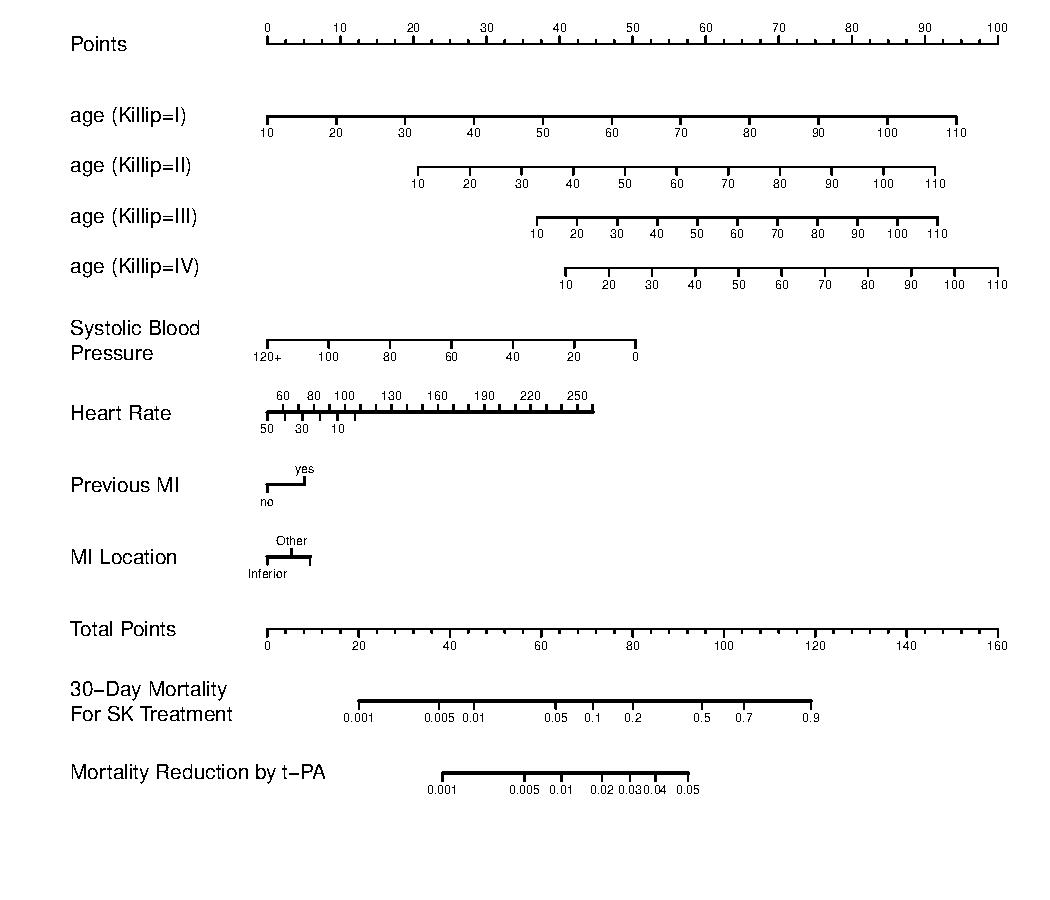
\includegraphics{ancova-gusto-nomogram-1} }

\caption[GUSTO-I nomogram]{Nomogram to predict SK - $t$--PA mortality difference, based on the difference between two binary logistic models.}\label{fig:ancova-gusto-nomogram}
\end{figure}


\subsubsection{Absolute Benefit on Survival Prob.}\sound{anc-13}
\bi
\item   Cox PH model
\item   Modeling can uncover time course of treatment effect
\item   $X_1$ = treatment, $A={X_{2},\ldots,X_{p}}$ adjustment
        variables
\item   Survival difference is \\ $S(t | X_{1}=1, A) - S(t | X_{1}=0, A)$
\\ $ = S(t | X_{1}=0, A)^{HR} - S(t | X_{1}=0, A)$
\begin{Schunk}
\begin{Sinput}
plot(0, 0, type="n", xlab="Survival for Control Subject",
     ylab="Improvement in Survival",
     xlim=c(0,1), ylim=c(0,.7))     # Fig. (*\ref{fig:ancova-hr-vs-surv}\ipacue*)
i <- 0
hr <- seq(.1, .9, by=.1)
for(h in hr) {
  i <- i + 1
  p <- seq(.0001, .9999, length=200)
  p2 <- p ^ h
  d <- p2 - p
  lines(p, d, lty=i)
  maxd <- max(d)
  smax <- p[d==maxd]
  text(smax,maxd+.02, format(h), cex=.6)
}
\end{Sinput}
\begin{figure}[htbp]

\centerline{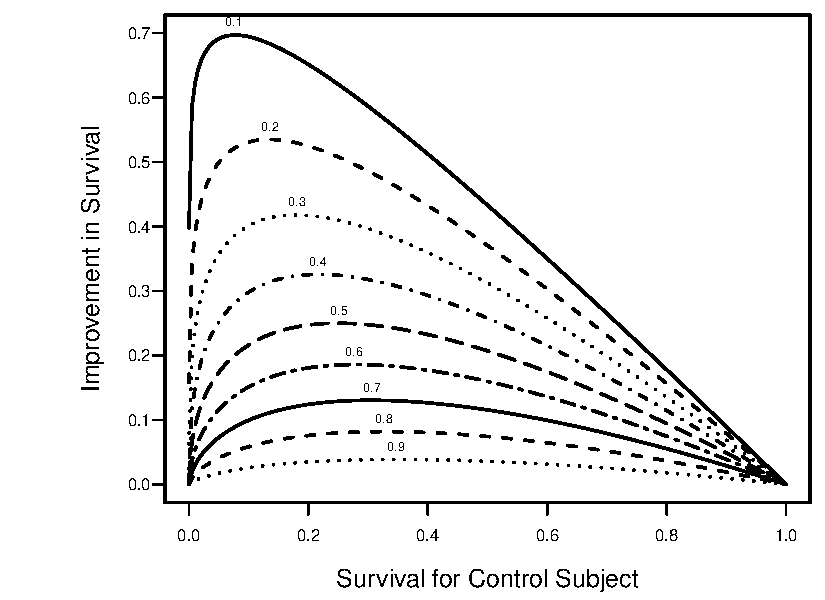
\includegraphics{ancova-hr-vs-surv-1} }

\caption[Baseline risk, hazard ratio, and absolute effect]{Relationship between baseline risk, relative treatment effect (hazard ratio --- numbers above curves) and absolute treatment effect.}\label{fig:ancova-hr-vs-surv}
\end{figure}
\end{Schunk}
\item See also \cite{ken07lim}.
\ei

\section{Cost--Effectiveness Ratios}\sound{anc-14}\disc{ancova-ceratio}
\bi
\item   Effectiveness E (denominator of C--E ratio) is always absolute
\item   Absolute treatment effectiveness varies greatly with patient
        characteristics
\item   \ra C--E ratio varies greatly
\item   A C--E ratio based on average E and average C
        may not apply to any existing patient!
\item   Need a model to estimate E
\item   C may also depend on patient characteristics
\begin{Schunk}
\begin{Sinput}
cost.life <- 2400 / delta / 1e6
plot(density(cost.life), xlab='Cost Per Life Saved, $M', main='',
     ylab='Probability Density', xlim=c(0, 6))    # Fig. (*\ref{fig:ancova-gusto-histcost}\ipacue*)
m <- 2400 / mean(delta) / 1e6
u <- par("usr")
arrows(m, u[3], m, 0, length=.1, lwd=2)
text(m,.01,'Cost using\n  average\n    reduction',srt=45,adj=0)
\end{Sinput}
\begin{figure}[htbp]

\centerline{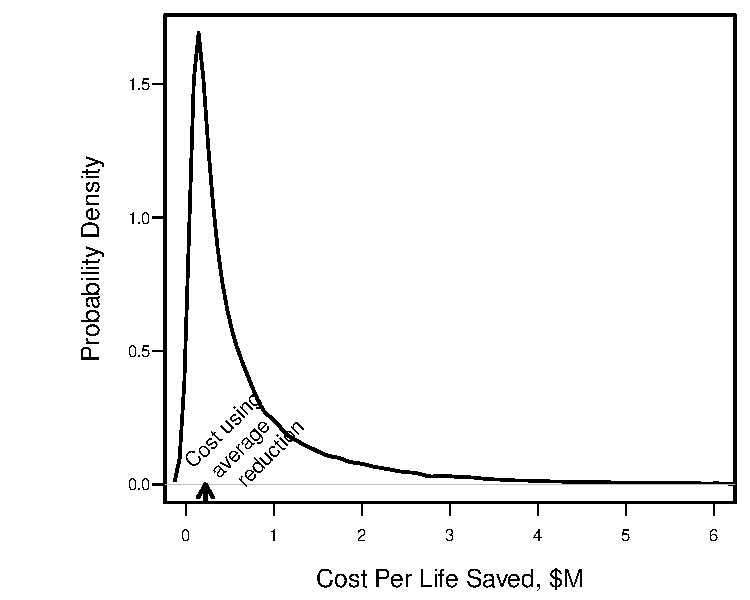
\includegraphics{ancova-gusto-histcost-1} }

\caption[Distribution of cost per life saved in GUSTO--I]{Distribution of cost per life saved in GUSTO--I}\label{fig:ancova-gusto-histcost}
\end{figure}
\end{Schunk}
\ei

\section{Treatment Contrasts for Multi--Site Randomized
  Trials}\disc{ancova-sites}
\bi
\item   Primary model: covariables, treatment, site main effects
\item   Planned secondary model to assess consistency of treatment
        effects over sites (add site $\times$ treatment interactions)
\item   Advantages for considering sites as random effects (or use
        penalized MLE to shrink site effects, especially for small sites).
        See \cite{and99tes} for a random effects Cox model and a
        demonstration that treatment effects may be inconsistent when
        non--zero site main effects are ignored in the Cox model.  See
        also \cite{yam99inv}.
\item   Types of tests / contrasts when interactions are included \ipacue
  \cite{sch00gen}:
    \bi
    \item   Type I: not adjusted for center
    \item   Type II: average treatment effect, weighted by size of
            sites \\
    \texttt{R} \co{rms} package command:
\begin{Schunk}
\begin{Sinput}
sites <- levels(site)
contrast(fit, list(treat='b', site=sites),
              list(treat='a', site=sites),
         type='average', weights=table(site))
\end{Sinput}
\end{Schunk}
    \item   Type III: average treatment effect, unweighted \\
\begin{Schunk}
\begin{Sinput}
contrast(fit, list(treat='b', site=sites),
              list(treat='a', site=sites), type='average')
\end{Sinput}
\end{Schunk}
    Low precision; studies are not powered for Type III tests.
    \ei

\item   Another interesting test: combined effects of treatment and
        site $\times$ treatment interaction; tests whether treatment
        was effective at {\em any} site.
\ei

\section{Statistical Plan for Randomized Trials}\disc{ancova-plan}
\bi
\item   When a relevant dataset is available before the trial begins,
        develop the model from the dataset and use the predicted value as a
        single adjustment covariable in the trial (Knaus et al.~\cite{kna93cli})
\item   Otherwise: CPMP Working Party: Finalize choice of model,
        transformations, interactions before merging treatment assignment
        into analysis dataset. \\
        Edwards \cite{edw99mod}: Pre--specify family of models that
        will be used, along with
        the strategy for selecting the particular model. \\
        Masked model derivation does not bias treatment effect.
\item CPMP guidance~\cite{cpmp04poi}
  \begin{quote}
    \begin{itemize}
\smaller
\item ``Stratification may be used to ensure balance of treatments across
covariates; it may also be used for administrative reasons.  The factors
that are the basis of stratification should normally be included as
covariates in the primary model.
\item Variables known a priori to be strongly, or at least moderately,
associated with the primary outcome and/or variables for which there is
a strong clinical rationale for such an association should also be
considered as covariates in the primary analysis.  The variables
selected on this basis should be pre-specified in the protocol or the
statistical analysis plan.
\item Baseline imbalance observed post hoc should not be considered an
appropriate reason for including a variable as a covariate in the
primary analysis.
\item Variables measured after randomization and so potentially affected by
the treatment should not normally be included as covariates in the
primary analysis.
\item If a baseline value of a continuous outcome measure is available, then
this should usually be included as a covariate.  This applies whether
the primary outcome variable is defined as the 'raw outcome' or as the
'change from baseline'.
\item Only a few covariates should be included in a primary analysis.
Although larger data sets may support more covariates than smaller ones,
justification for including each of the covariates should be
provided. (???)
\item In the absence of prior knowledge, a simple functional form (usually
either linearity or dichotomising a continuous scale) should be assumed
for the relationship between a continuous covariate and the outcome
variable. (???)
\item The validity of the model assumptions must be checked when assessing
the results.  This is particularly important for generalized linear or
non-linear models where mis-specification could lead to incorrect
estimates of the treatment effect.  Even under ordinary linear models,
some attention should be paid to the possible influence of extreme
outlying values.
\item Whenever adjusted analyses are presented, results of the treatment
effect in subgroups formed by the covariates (appropriately categorised,
if relevant) should be presented to enable an assessment of the validity
of the model assumptions. (???)
\item Sensitivity analyses should be pre-planned and presented to
investigate the robustness of the primary results.  Discrepancies should
be discussed and explained.  In the presence of important differences
that cannot be logically explained-for example, between the results of
adjusted and unadjusted analyses-the interpretation of the trial could
be seriously affected.
\item The primary model should not include treatment by covariate
interactions.  If substantial interactions are expected a priori, the
trial should be designed to allow separate estimates of the treatment
effects in specific subgroups.
\item Exploratory analyses may be carried out to improve the understanding
of covariates not included in the primary analysis, and to help the
sponsor with the ongoing development of the drug.
\item A primary analysis, unambiguously pre-specified in the protocol or
statistical analysis plan, correctly carried out and interpreted, should
support the conclusions which are drawn from the trial.  Since there may
be a number of alternative valid analyses, results based on
pre-specified analyses will carry most credibility.''
\end{itemize}
  \end{quote}

\quoteit{In confirmatory trials, a model is pre-specified, and it is
necessary to pretend that it is true.  In most other statistical
applications, the choice of model is data--driven, but it is necessary
to pretend that it is not.}{\citet{edw99mod}}

        See also Siqueira and Taylor~\cite{sig99tre}.
\item   Choose predictors based on expert opinion \ipacue
\item   Impute missing values rather than discarding observations
\item   Keep all pre--specified predictors in model, regardless of $P$--value
%\item  Stepwise variable selection will ruin standard errors,
%       confidence limits, $P$--values, etc.
%\item  Extract maximum information from (objective) continuous
%       predictors using regression splines or nonparametric smoothers
\item   Use shrinkage (penalized maximum likelihood estimation) to
        avoid over--adjustment
%\item  Shrink regression coefficients for adjustment variables
%       (but not treatment!) with maximum validation of model in mind
%       (AIC) (Verweij and van Houwelingen 1994)
%\item  Maximize penalized log likelihood function: \\
%$\log L - \frac{1}{2} \lambda \sum_{i=1}^{p} (s_{i}\beta_{i})^{2}$
%\item  Generalize: $\log L - \frac{1}{2} \lambda \beta' P \beta$
%\item  Categorical predictors are penalized differently
%\item  $\log L$ is ordinary log like.  \\
%       $s$ are scale factors (e.g., predictor S.D.) \\
%        $\lambda$ is penalty parameter
%\item  Optimum shrinkage will tell the statistician how many
%       regression d.f. the dataset can reliably support
%\item  Use the bootstrap to validate the model using all patients
\item Some guidance for handling missing baseline data in RCTs is in
  White \& Thompson~\cite{whi05adj}
\ei

\subsection{Sites vs.\ Covariables}\disc{ancova-sites}
\bi
\item Site effects (main or interaction) are almost always trivial in
  comparison with patient-specific covariable effects
\item It is not sensible to include site in the model when important
  covariables are omitted
\item The most logical and usually the most strong interaction with
  treatment is not site but is the severity of disease being treated
\ei

\subsection{Covariable Adjustment vs.\ Allocation Based on
  Covariates}\ipacue \disc{ancova-plan}
\quoteit{The decision to fit prognostic factors has a far
more dramatic effect on the precision of our inferences than the choice
of an allocation based on covariates or randomization approach and one
of my chief objections to the allocation based on covariates approach
is that trialists have tended to use the fact that they have balanced
as an excuse for not fitting.  This is a grave
mistake.}{\citet{sen04con}, p.\ 3748; see also \citet{sen10com}}

\quoteit{My view \ldots was that the
form of analysis envisaged (that is to say, which factors and
covariates should be fitted) justified the allocation and \emph{not
vice versa}.}{\citet{sen04con}, p.\ 3747}

\section{Summary}
\quoteit{The point of view is sometimes
defended that analyses that ignore covariates are superior because
they are simpler. I do not accept this.  A value of $\pi=3$ is a
simple one and accurate to one significant figure \ldots However very few
would seriously maintain that if should generally be adopted by
engineers.}{\citet{sen04con}, p.\ 3741}

\bi
\item  As opposed to simple treatment group comparisons, modeling can
   \bi
   \item   Improve precision (linear, log--linear models)
   \item   Get the ``right'' treatment effect (nonlinear models)
   \item   Improve power (almost all models)
   \item   Uncover outcome patterns, shapes of effects
   \item   Test/estimate differential treatment benefit
   \item   Determine whether some patients are too sick or too well to benefit
   \item   Estimate absolute clinical benefit as a function of
           severity of illness
   \item   Estimate meaningful cost--effectiveness ratios
   \item   Help design the next clinical trial (optimize risk
           distribution for maximum power)
   \ei
\item  Modeling strategy must be well thought--out \ipacue
   \bi
   \item   Not ``data mining''
   \item   Not done to optimize the treatment $P$--value
   \ei
\ei

\section{Notes}
From a posting by Harrell to the Medstats google group on 19Jan09:
{\small
I think it is most important to decide what it is you want to
estimate, and then formulate a model that will accomplish that.
Unlike ordinary linear models, which provide unbiased treatment
effects if balanced covariates are mistakenly omitted from the model
in an RCT, most models (such as the Cox PH model) result in biased
treatment effects even when there is perfect balance in covariates, if
the covariates have nonzero effects on the outcome.  This is another
way of talking about residual outcome heterogeneity.

If you want to estimate the effect of variable $X$ on survival time,
averaging over males and females in some strange undocumented way, you
can get the population averaged effect of $X$ without including sex in
the model.  Recognize however this is like comparing some of the males
with some of the females when estimating the $X$ effect.  This is seldom
of interest.  More likely we want to know the effect of $X$ for males,
the effect for females, and if there is no interaction we pool the two
to more precisely estimate the effect of $X$ conditional on sex.

Another way to view this is that the PH assumption is more likely to
hold when you condition on covariates than when you don't.  No matter
what happens though, if PH holds for one case, it cannot hold for the
other, e.g., if PH holds after conditioning, it cannot hold when just
looking at the marginal effect of X.
}
%\nocite{alt90ran,beg90sig,sen94tes,rob91som,ste00cli,gai84bia,gai86adj,gai88tes,lag84pro,mor86omi,for95mod,aka97pow,sch83sam,sar96hie,and99tes,cpm95bio,har96mul,ver94pen,hau91,kna93cli,ich98,kal97tre,lew95sta,mac98whi,sen97sta,rms,for02rol,poc02sub,her04cov,aus10sub}

\def\apacue{0}
